%% LyX 2.3.5.2 created this file.  For more info, see http://www.lyx.org/.
%% Do not edit unless you really know what you are doing.
\documentclass[english]{article}
\PassOptionsToPackage{natbib=true}{biblatex}
\usepackage{fourier}
\usepackage[T1]{fontenc}
\usepackage[utf8]{inputenc}
\usepackage{geometry}
\geometry{verbose,tmargin=2cm,bmargin=2cm,lmargin=2cm,rmargin=2cm}
\usepackage{babel}
\usepackage{graphicx}
\usepackage[unicode=true]
 {hyperref}

\makeatletter
%%%%%%%%%%%%%%%%%%%%%%%%%%%%%% User specified LaTeX commands.
%\usepackage[style=numeric,backend=biber,maxbibnames=99]{biblatex}
\usepackage{hyperref}

\AtBeginDocument{
  \def\labelitemii{\(\ast\)}
  \def\labelitemiii{\(\star\)}
}

\makeatother

\usepackage[style=authoryear,maxbibnames=99]{biblatex}
\addbibresource{papers.bib}
\begin{document}
\title{Paper summaries}
\maketitle

\section{\protect\href{https://docs.google.com/presentation/d/1m4Z3RJDueaKMvCO-cb_Ia51nTW6-OSE9hXVPy1l1-_I/edit?usp=sharing}{On the Automatic Generation of Medical Imaging Reports}
\citep{baoyu_jing2018}}

\subsection{Introduction}

The reading and interpretation of medical images are usually conducted
by specialized medical professionals. Report writing can be error-prone
for inexperienced physicians, and time-consuming and tedious for experienced
physicians. \\
Several challenges need to be addressed:
\begin{enumerate}
\item A complete report consists of multiple heterogeneous sources of information
\item Localize image regions and attach the right description to them 
\item Descriptions in reports are usually long, with multiple sentences
\end{enumerate}
The proposed solutions are:
\begin{enumerate}
\item A \textbf{multi-task learning framework} for simultaneous prediction
of tags and text generation
\item A \textbf{Co-attention mechanism: }simultaneous attention to images
and predicted tags; explores synergistic effects of visual and semantic
information 
\item A \textbf{Hierarchical LSTM: }Leverages compositional nature of reports:
first generates high-level topics, then fine-grained descriptions
from each one
\end{enumerate}
\begin{figure}
\begin{centering}
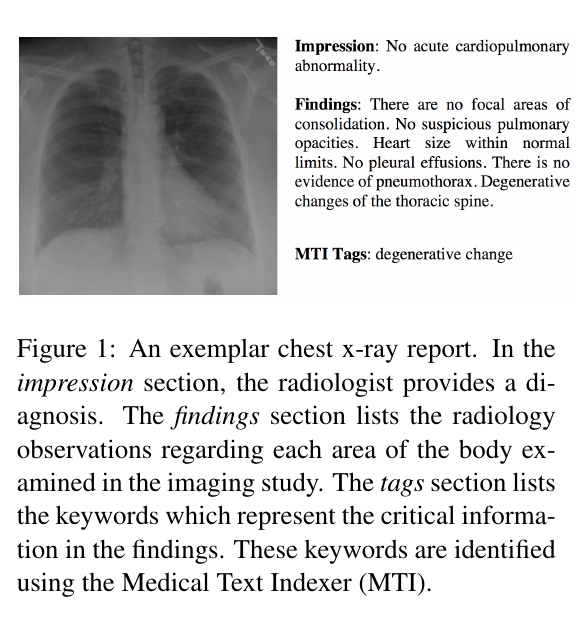
\includegraphics[scale=0.5]{images/baoyu_jing_report}
\par\end{centering}
\caption{Sample report from IU X-ray}

\end{figure}


\subsection{Methods and Architecture}

An image is divided into regions, and a CNN encoder is used to learn
visual features for these patches. These features are fed into a \emph{multi-label
classifier}, from which tags are predicted. These tags are transformed
into \emph{semantic feature vectors }by a custom embedding. Both visual
and semantic features are fed into the co-attention module, which
produces a combined \emph{context vector, }which \textbf{simultaneously
captures the visual and semantic information of this image.} 

The decoding and caption generation process is performed by the hierarchical
LSTM, which leverages the compositional structure of a medical report
(each sentence focusing on one specific topic). The sentence LSTM,
using the context vector, first generates a sequence of high-level
topic vectors representing sentences. 

\begin{figure}
\begin{centering}
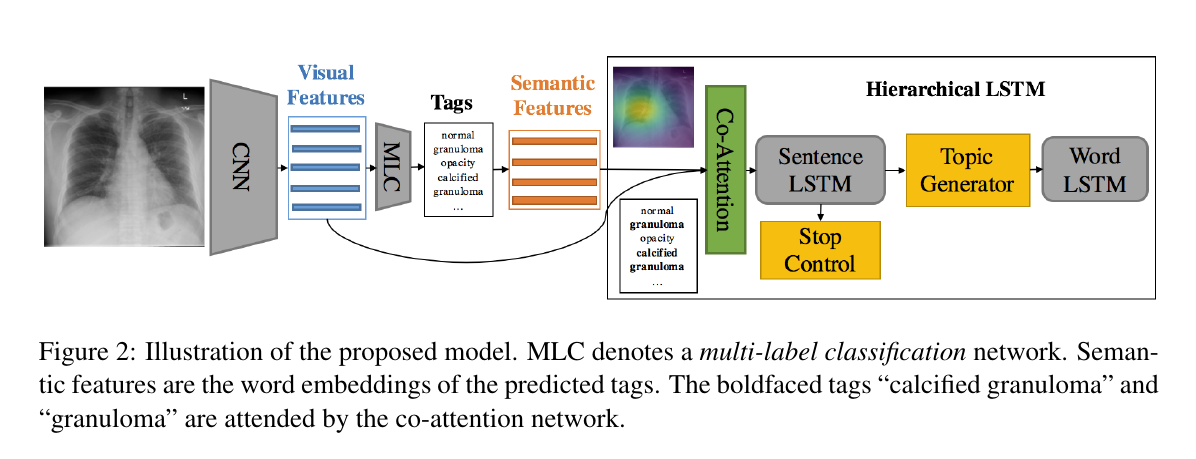
\includegraphics[scale=0.5]{images/baoyu_jing_architecture}
\par\end{centering}
\caption{Architecture}
\end{figure}

\printbibliography

\end{document}
